Robots operating in unstructured, stochastic environments such as a
factory floor or a kitchen face a difficult planning problem due to
the large state space and the very large set of possible
tasks~\citep{bollini12,knepper13}.  A powerful and flexible robot such
as a mobile manipulator in the home has a very large set of possible
actions, any of which may be relevant depending on the current goal
(for example, robots assembling furniture~\citep{knepper13} or baking
cookies~\citep{bollini12}.)  When a robot is manipulating objects in
an environment, an object can be placed anywhere in a large set of
locations.  The size of the state space increases exponentially with
the number of objects, which bounds the placement problems that the
robot is able to expediently solve.  Depending on the reward function
(which is unknown before runtime), any of these states and actions may
be relevant to the solution, but for any specific reward function,
most of them are irrelevant.  For instance, when making brownies, the
oven and flour are important, while the soy sauce and saut\'{e} pan
are not.  For a different task, such as stir-frying broccoli, the
robot must use a different set of objects and
actions. 
\begin{figure}
\centering
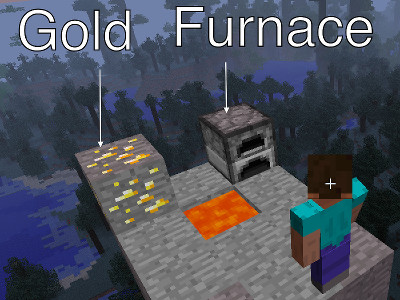
\includegraphics[width=0.2\linewidth]{figures/smelt_small.jpg}
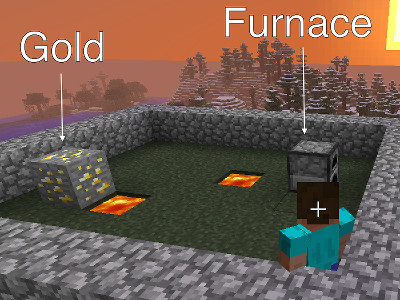
\includegraphics[width=0.2\linewidth]{figures/smelt_large.jpg}
\caption{Two different versions of the gold smelting task.
  The task on the right is only able to be solved after learning in the
  simpler version of the left because the state space is too large.
  \label{fig:example}}
\end{figure}

To confront this state-action space explosion, prior work has explored
adding knowledge to the planner, such as options~\cite{sutton99} and
macro-actions~\cite{Botea:2005kx,Newton:2005vn}.  However, while these
methods can allow the agent to search more deeply in the state space,
they add non-primitive actions to the planner which {\em increase} the
branching factor of the state-action space.  The resulting augmented
space is even larger, which can have the paradoxical effect of
increasing the search time for a good policy~\cite{Jong:2008zr}.
%Deterministic forward-search algorithms like hierarchical task
%networks (HTNs)~\citep{Nau:1999:SSH:1624312.1624357}, and temporal
%logical planning
%(TLPlan)~\citep{Bacchus95usingtemporal,Bacchus99usingtemporal}, add
%knowledge to the planner that greatly increases planning speed, but do
%not generalize to stochastic domains. Additionally, the knowledge
%provided to the planner by these methods is quite extensive, reducing
%the agent's autonomy and must be manually supplied by the designer.

To address these issues, we learn action
priors that are conditioned on the current state and goal
from training MDPs drawn from a distribution. Because we
condition on both the state and goal description, we refer to this
goal-based action prior as a knowledge base of {\em affordances}.
Affordances enable the robot to prune irrelevant actions from the 
search space on a
state-by-state basis based on the agent's current goal and focus on
the most promising parts of the state space. Actions are determined
to be irrelevant when according to the affordance model they
have a low probability of being optimal.

%Our experiments
%demonstrate that affordances provide dramatic improvements for a
%variety of planning tasks compared to baselines in simulation, and are
%applicable across different state spaces. As a baseline, we
%compare planning with learned affordances to manual afforances defined
%by an expert. While the manual affordances outperform
%a baseline planning algorithm without affordances, the learned
%affordances yield even better performance.



%we augment an Object Oriented Markov Decision
%Process (OO-MDP) with a specific type of action prior conditioned on
%the current state and an abstract goal description.  Because we
%condition on both the state and goal description, we refer to this
%goal-based action prior as a knowlege base of {\em affordances}.  We
%rigorously formalize the notion of affordances as a prior on actions
%conditioned on features of the current state as well as the robot's
%goal.  Affordances enable the robot to prune irrelevant actions on a
%state-by-state basis based on the agent's current goal and focus on
%the most promising parts of the state space.  Affordances can be
%specified by hand or alternatively learned through experience in
%related problems, making them a concise, transferable, and learnable
%means of representing useful planning knowledge. Our experiments
%demonstrate that affordances provide dramatic improvements for a
%variety of planning tasks compared to baselines in simulation, and are
%applicable across different state spaces.  Moreover, while manually
%provided affordances outperform baselines, affordances learned through
%experience yield even greater improvements.We conduct experiments in
%the game Minecraft, which has a very large state-action space, and on
%a real-world robotic cooking assistant.  Figure~\ref{fig:example}
%shows an example of two problems from the same domain in the game
%Minecraft; the agent learns on randomly generated problems and tests
%on new problems from the same domain that it has never previously
%encountered.


To learn affordances, we sample a set of of training worlds from the
domain ($W$), for which the optimal policy, $\pi$, may be tractably
computed using existing planning methods. Then, we compute the maximum
likelihood estimate of the parameter vector $\theta_i$ for each action
using the policy. In our experiments, we use a Naive Bayes model
in which the probability of state features are treated as independent given
the optimal action.
During the learning phase, the agent learns which
actions are useful under different conditions. At test time, the agent
will see different, randomly generated worlds from the same domain,
and use the learned affordances to increase its speed at finding a
policy. 
For simplicity, our learning process uses a strict separation
between training and test; after learning is complete our model
parameters remain fixed for the entire test time. 

We evaluate our approach using the game Minecraft.  Minecraft is a 3-D
blocks game in which the user can place, craft, and destroy blocks of
different types.  Minecraft's physics and action space allow users to
create complex systems, including logic gates and functional
scientific graphing
calculators\footnote{https://www.youtube.com/watch?v=wgJfVRhotlQ}.
Minecraft serves as a model for robotic tasks such as cooking
assistance, assembling items in a factory, object retrieval, and
complex terrain traversal.
Our experiments consisted of five common tasks in
Minecraft, including constructing bridges over trenches, smelting
gold, tunneling through walls, basic path planning, and digging to
find an object. Figure~\ref{fig:example} shows two scenes
from Minecraft that were drawn from our distribution of MDPs.  
We tested on randomized worlds of varying size and
difficulty. The generated test worlds varied in size from tens of
thousands of states to hundreds of thousands of states.  The agent
learned affordances from a training set consisting of 25 simple state
spaces of each map type (100 total maps), each approximately a
1,000-10,000 state world. We conducted all tests with a single
knowledge base. Learning this knowledge base took approximately one
hour run in parallel on a computing grid.


We use Real-Time Dynamic Programming (RTDP)~\cite{barto95} as our
baseline planner, a sampling-based algorithm that does not require the
planner to visit all states. We compare RTDP with learned
affordance-aware RTDP (LA-RTDP), and expert-defined affordance-aware
RTDP (EA-RTDP), in which the action priors are specified by an expert. 
We terminated each planner when the maximum change in
the value function was less than 0.01 for 100 consecutive policy
rollouts, or the planner failed to converge after 1000 rollouts.  The
reward function was $-1$ for all transitions, except transitions to
states in which the agent was in lava, where we set the reward to
$-10$. The goal was set to be terminal and the discount factor was
$\gamma = 0.99$.  To introduce non-determinism into our problem,
movement actions (move, rotate, jump) in all experiments had a small
probability (0.05) of incorrectly applying a different movement
action.  This noise factor approximates noise faced by a physical
robot that attempts to execute actions in a real-world domain and
can affect the optimal policy due to the existence of lava pits
that the agent can fall into. Figure~\ref{fig:average_results}
summarizes the testing performance for all planning algorithms
in terms of average number of Bellman updates in RTDP, the average
cost of the policy found after planning termination, and the average
amount of CPU time. In all cases, planning with learned affordances
performed best, then expert performance, and finally the baseline
performed worst. Although RTDP converges to the optimal policy in the
limit, its average policy cost was worse than the other methods because
in many cases it was not able to find a reasonable policy in the
amount of planning time allotted.


% -- Figure: Average results --
\begin{figure}[t]
%\begin{figure}
\centering
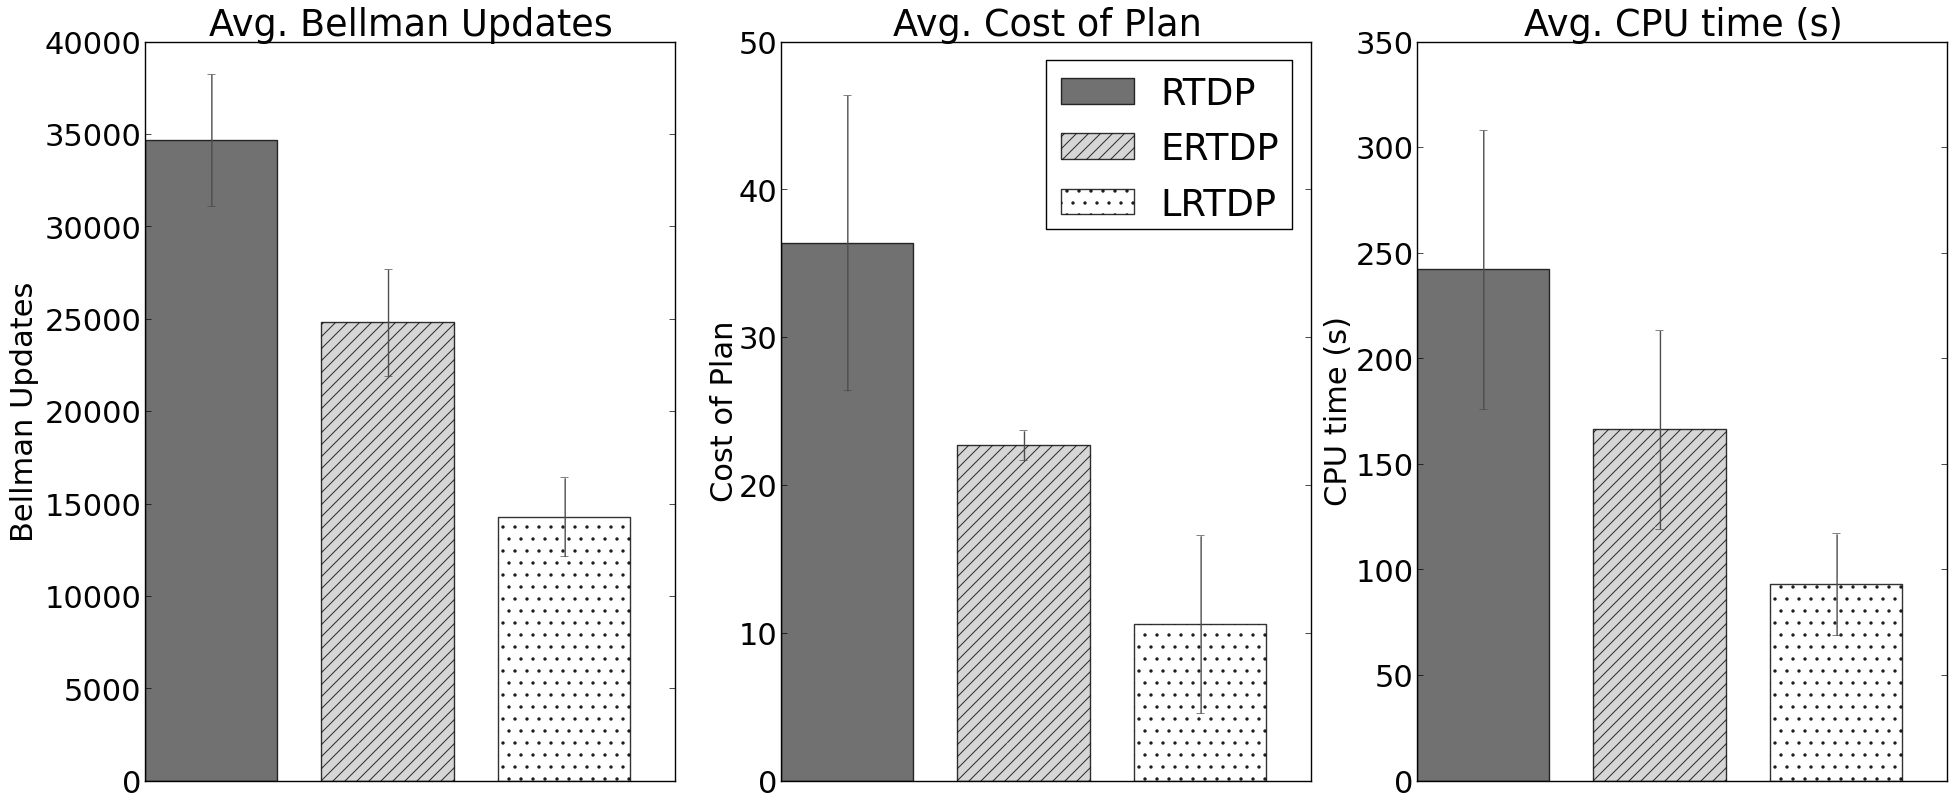
\includegraphics[width=0.3\linewidth]{figures/average_results_cropped.png}%
%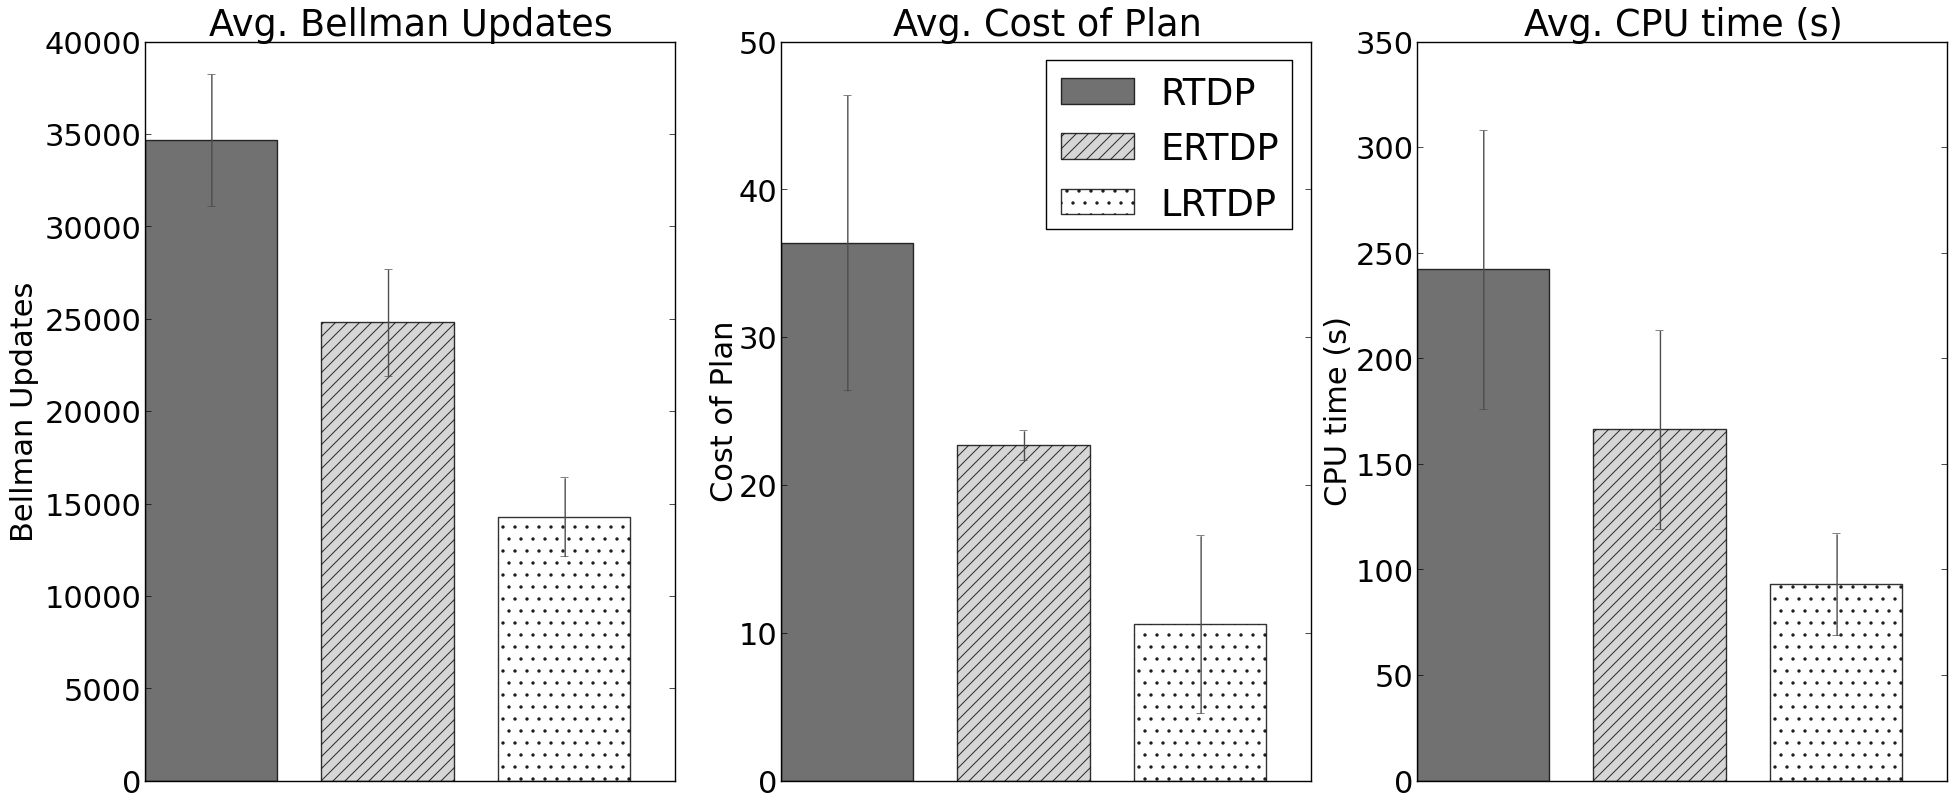
\includegraphics[scale=0.18]{figures/average_results_cropped.png}%
\caption{Average results from all maps.}
\label{fig:average_results}
\end{figure}
%\end{figure}

